% Appendix A

\chapter{Batches fabrication details} % Main appendix title

\label{AppendixA} % For referencing this appendix elsewhere, use \ref{AppendixA}

\section{Process parameters}
\label{ppa}
Dimensions of the cubic and cylindrical specimens are noted in accordance with figure \ref{fig:cc}. [AJOUTER DERNIER BATCH]\\
 %\begin{center}
\begin{table}[ht]
\noindent\makebox[\textwidth]{\begin{tabular}{|c|c|c |c |c|c|c|}

    \hline
  Batch name & Contour & Type & Dimensions [mm] &Specimen name & $\frac{P}{P_{max}} [-]$ & $v_s [\frac{mm}{s}]$\\
  \hline
  \hline
  X200-171024 & No & Cubic & L=10& 1 & 0.85 & 900\\
  & &   & & 2 &  & 1000\\
  & &   & & 3&  & 1059\\
  & &  & & 4&  & 1500\\
  & &  & & 5& 1 & 900\\
  & &  & & 6&  & 1059\\
  & & & & 7, 7a, 7b & 0.75 & 1200\\
  & & & & 8, 8a, 8b& & 900\\
\hline  
  X200-180109 & No&Cubic & L=10 & 7c,...7q (15 spec.)& 0.75 &1200\\
  & & & & 8c,...8q (15 spec.)  & & 900\\
\hline  
  X200-180220 & No & Cubic & L=5 & TT150-2 & 0.75 & 1200\\
  & &  & & TT200-2 &  &\\
  & &  & & TT300-2 &  &\\
  & &  & & TT300-2-plaque &  &\\
  & &  & & TT150-2-real &  &\\
  & &  & & TT200-2-real &  &\\
  & &  & & TT250-2-real &  &\\
  & &  & & TT300-2-real &  &\\
\hline  
  X200-180222 & No & Cubic & L=10 &12& 0.75 & 1200\\
  & &  & &13 &  &\\
\hline  
  X200-180228  & Yes & Cylindrical & D=6, H=2 &1 & 0.75 & 1200\\
  & &  &  & 2&  & \\
  & &  &  & 3 &  & \\
\hline  
  X200180313 & Yes & Cylindrical & D=6, H=10&1& 0.75 & 1200\\
    & &    & &2 & &  \\
    & &  &D=12, H=10 &3& &  \\
    & & & &4 & & \\
\hline  
  X200-180319  & No & Cubic & L=10 & cub 1 & 0.75 & 1200\\
  & &  & & cub 2 & &\\
  & &  & & cub 3 & &\\
  & & & & cub 4 & &\\
  & & & & cub 5 & &\\
  & & &  L=5& TT300-1-real &  &\\ 
  & Yes &  Cylindrical & D=6, H=10&cyl 1   &  & \\
    & &  & &cyl 2 & & \\
    & &  & D=12, H=10 &cyl 3 & & \\
    & &  &  &cyl 4  & & \\

    \hline

\end{tabular}}
\caption[Manufacturing process parameters]{Manufacturing process parameters}
\label{table:Pparam}
\end{table}
 %\end{center}

\begin{figure}[ht]
\centering
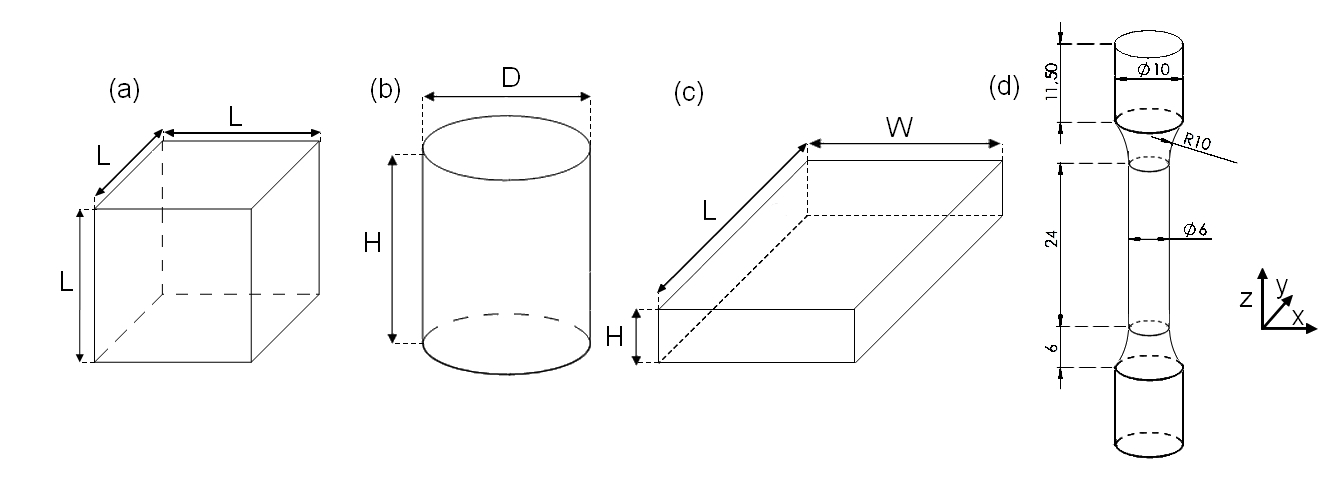
\includegraphics[scale=0.58]{Images/cc}
\caption[Dimensions notations for (a) cubic specimens (b) cylindrical specimens]{Dimensions notations for (a) cubic specimens (b) cylindrical specimens}
\label{fig:cc}
\end{figure}

 
\section{Specimens positioning, fabrication orders and sintering times}
\label{mda}
\subsection{Batch X200-171024}

\begin{figure}[ht]
\centering
\noindent\makebox[\textwidth]{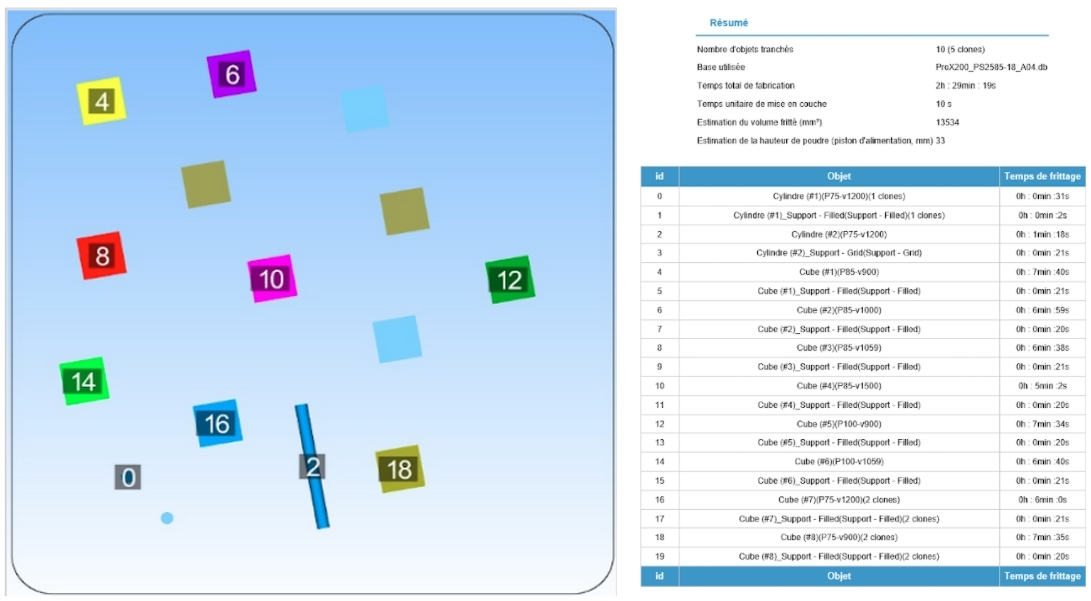
\includegraphics[scale=0.58]{Images/171024-cad}}
\decoRule
\caption[Specimens positions, order of fabrication and sintering times for batch X200-171024]{Specimens positions, order of fabrication and sintering times for batch X200-171024}
\label{fig:171024-cad}
\end{figure}

\begin{figure}[ht]
\centering
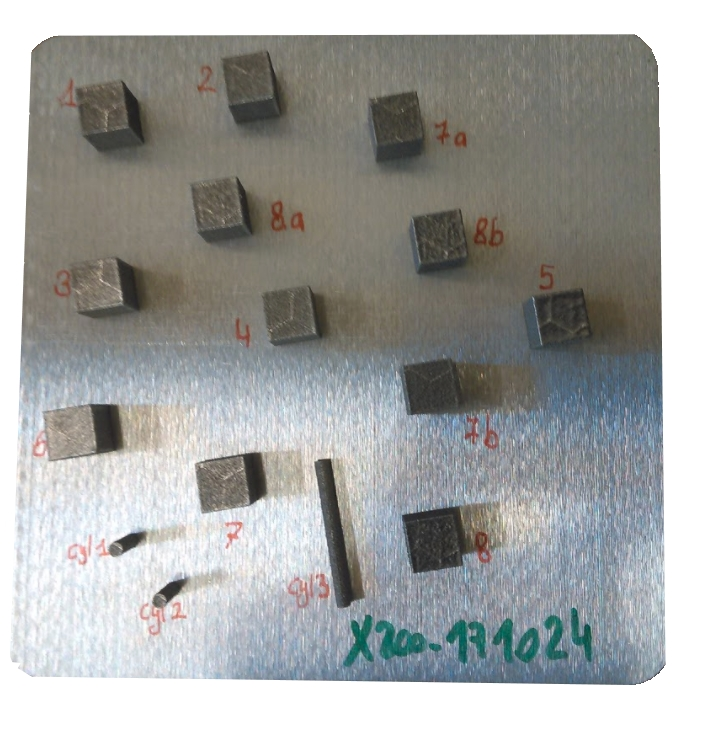
\includegraphics[scale=0.45]{Images/171024-real}
\decoRule
\caption[Photography of the manufacturing plate after completion of the fabrication of batch X200-171024]{Photography of the manufacturing plate after completion of the fabrication of batch X200-171024}
\label{fig:171024-real}
\end{figure}


\subsection{Batch X200-180109}

... ... ...

\subsection{...Other batches}